%% Bemærk:
%%          Resten af rapporten følger en stil hvor indledninger skrives
%%          med \sffamlily-typen. Denne stil bør også følges her.
%%
{\sffamily
I denne sektion vil vi teste den naive løsning. Ved at se om den sortere
de rigtige regioner væk og om løsningen opfører sig på samme måde som vi
har håbet på. Det vil vi gøre ved først at se på nogle fabrikeret
testbilleder, for at se om den naive løsning virker efter hensigten og
bagefter vil vi teste på malerierne for at se om den naive løsning kan
bruges i praksis.
}
  
\subsection{Afprøvning på testbilleder}
Vi vil teste på de samme testbilleder som i sideste afsnit, samt et nyt
testbilleder, som blev brugt i forklaringen af den naive metodes. De fire
billeder som vi har valgt at teste kan ses i afsnit \ref{region_detektor}
og billedet \ref{naiv_masse_original} hvor en grå kasse rundt om en
region, betyder at den er valgt til at ligge i det gyldne snit af den
naive metode. 

Det første billede \ref{naiv_blob1}, har fem regioner. Kun tre af
dem blev fundet under udtrækningen af regioner, vores naive løsning har så
sorteret baggrundensregionen og den øverste region i snittet væk, da
ingen af de to regioners kanter ikke ligger i snittets marginer og
overholder regionerne ikke defination \ref{def_naiv} . 

\begin{figure}[!h]
	\begin{center}
        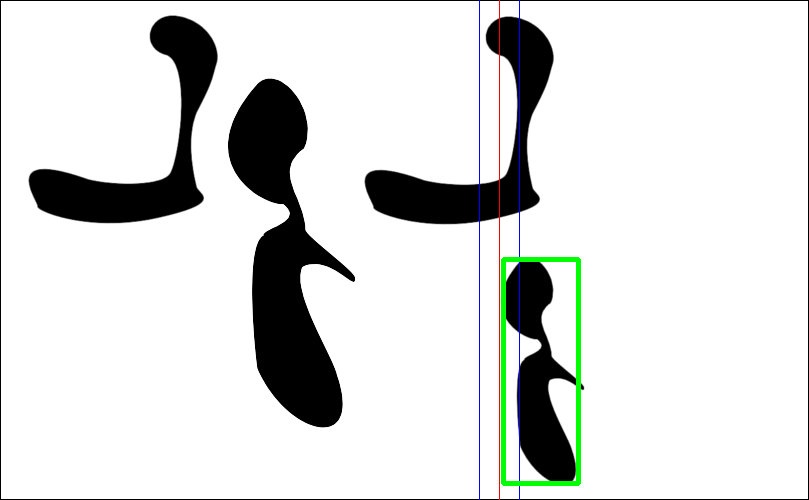
\includegraphics[angle=0,width=0.55\textwidth]{afsnit/afprovning/billeder/naive_losning/naiv_blob1.png}
	\end{center}       
	\caption{Naive algoritme finder en ud af fem regioner.}	
	\label{naiv_blob1}
\end{figure}

På det andet billede \ref{naiv_blob2}, er alle regionerne blevet sorteret væk, også
den lille, da den er for lille, og overholdet derfor ikke definition
\ref{def_interessant} b. 

\begin{figure}[!h]
	\begin{center}
       	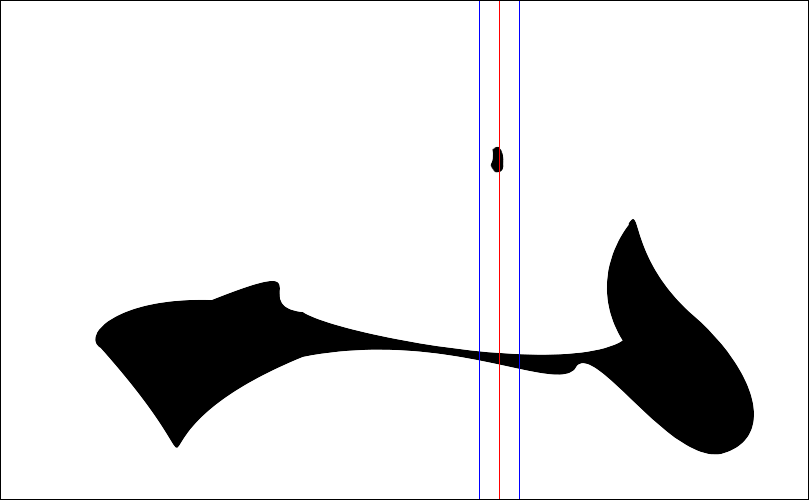
\includegraphics[angle=0,width=0.55\textwidth]{afsnit/afprovning/billeder/naive_losning/naiv_blob2.png}
	\end{center}
	\caption{Værgen den lille region eller den store er fundet.} 
   	\label{naiv_blob2}
\end{figure}

I testbilledet \ref{naive_hoisont1}, sortere algoritmen
himlen fra, da den krydser marginen lidt, men jorden tages med. 

\begin{figure}[!h]
	\begin{center}
       	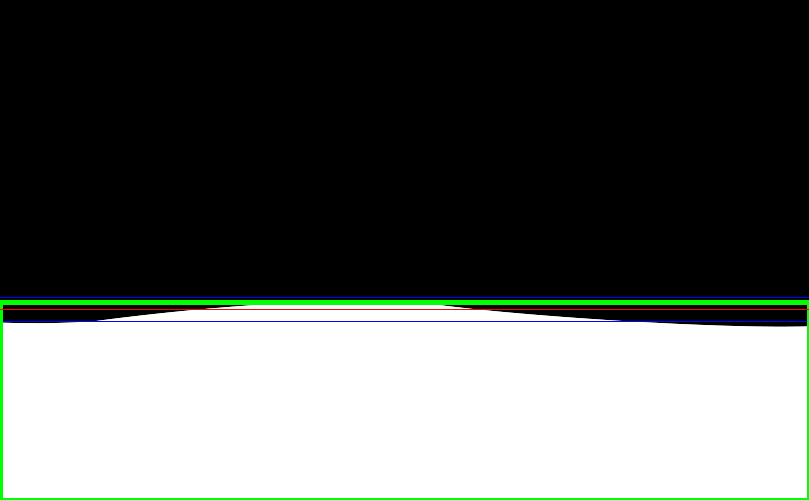
\includegraphics[angle=0,width=0.55\textwidth]{afsnit/afprovning/billeder/naive_losning/naiv_hoisont1.png}
	\end{center}
	\caption{Kun den nederste horisont er fundet} 
   	\label{naive_hoisont1}
\end{figure}

\clearpage

\subsection{Afprøvning på malerier}
Vi afprøver den naive algoritme på seks malerier, først på tre malerier,
hvor regions detektoren virker efter vores hensigt og så på tre
malerier, hvor region detektoren ikke virker. Beskrivelsen af hvad der
sker i billedet vil står i billedbeskrivelse.


\begin{figure}[h!!]
	\begin{center}
		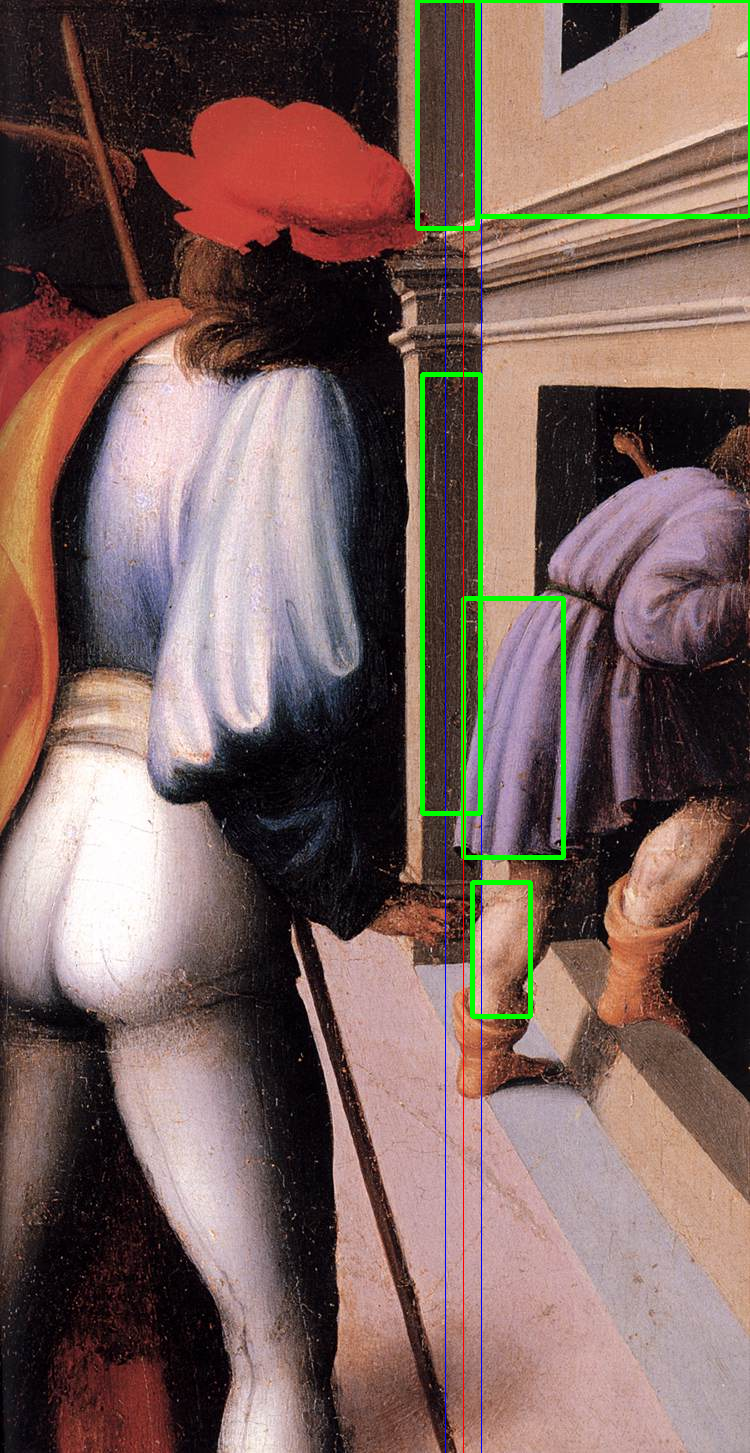
\includegraphics[scale=0.3,angle=0]{afsnit/afprovning/billeder/naive_losning/naiv_kfarver_sdetaljer.png}
	\end{center}
	\caption[]{Fem ud af de seks store regioner fra figur
	\ref{GRD_virker1} valgt til at ligge i snittet, skoene er for små til
	at blive taget med i betragtningen.}
	\label{naiv_kfarver_sdetaljer}
\end{figure}

\begin{figure}[h!!]
	\begin{center}
		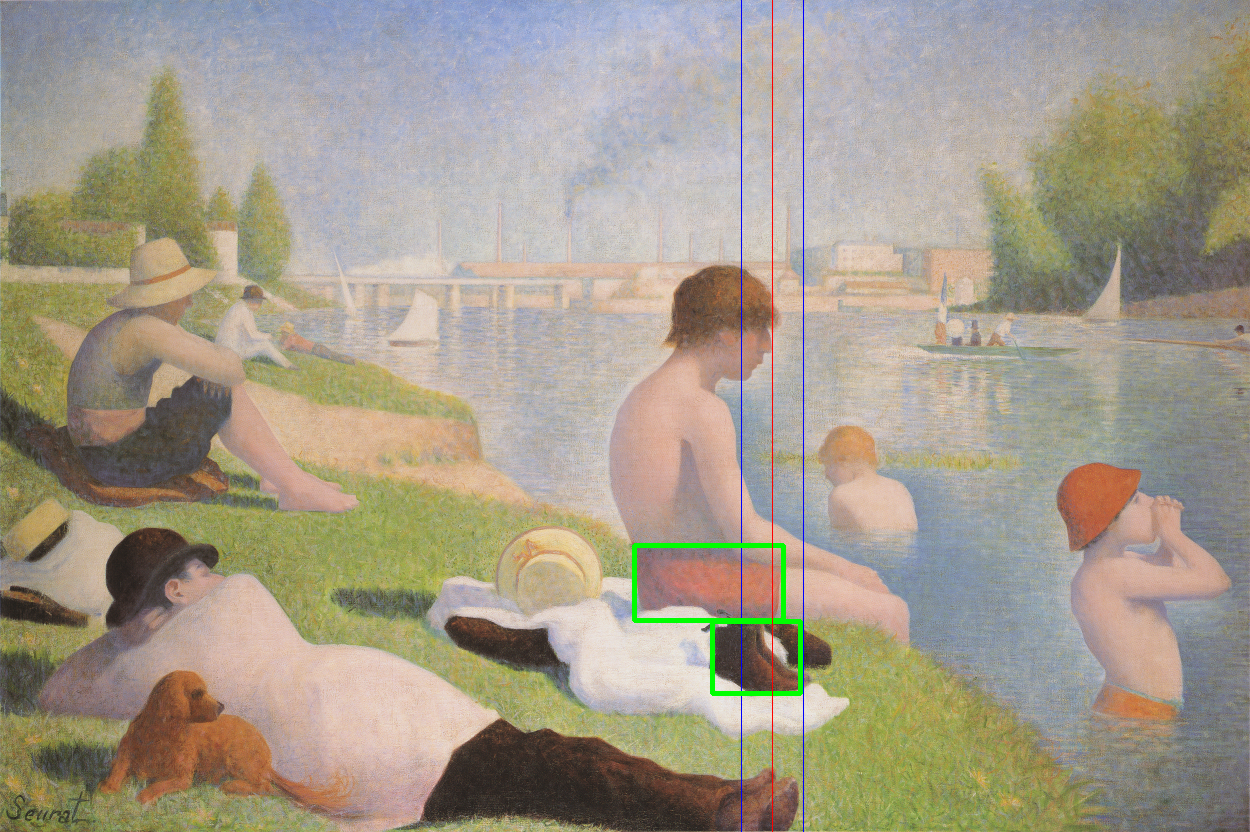
\includegraphics[scale=0.3,angle=0]{afsnit/afprovning/billeder/naive_losning/naiv_mfarver_mdetaljer.png}
	\end{center}
	\caption[]{Bukserne og skoene er tager med af den naive løsning, men
	drengen er sorteret væk da han krydser snittet}
	\label{naiv_mfarver_mdetaljer}
\end{figure}

\begin{figure}[h!!]
	\begin{center}
		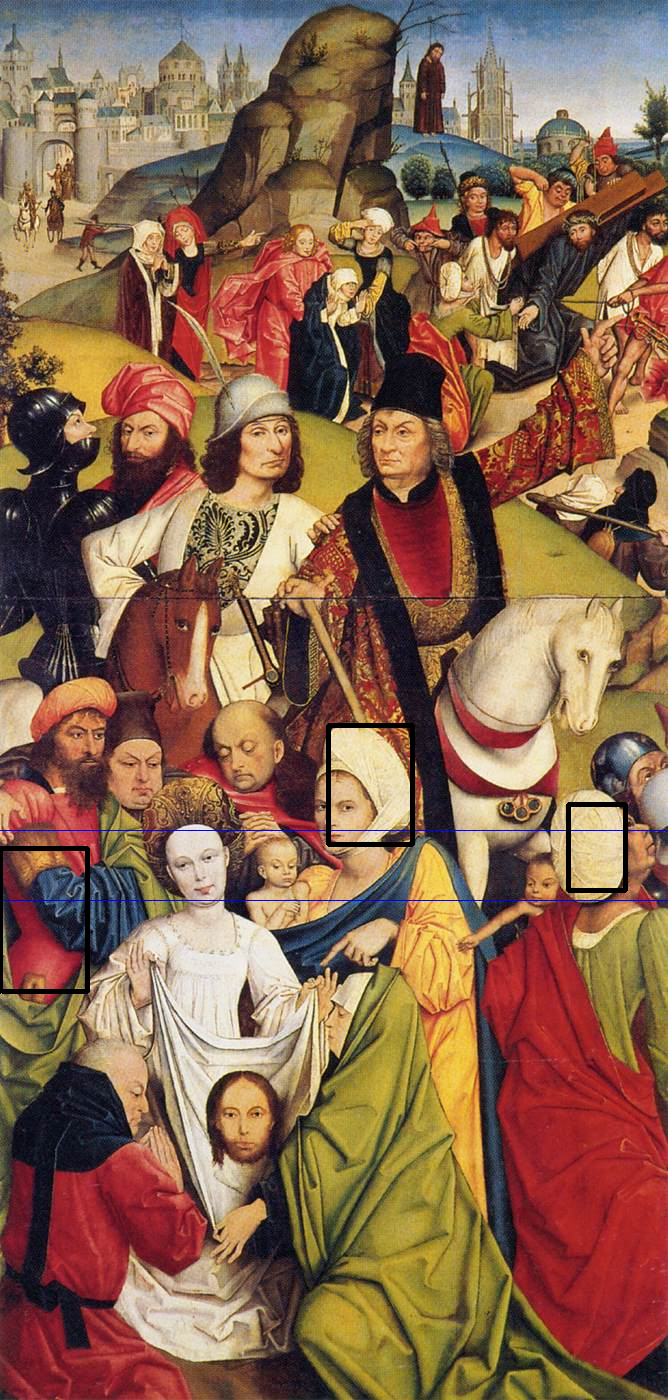
\includegraphics[scale=0.3,angle=0]{afsnit/afprovning/billeder/naive_losning/naiv_kfarver_kdetaljer.png}
	\end{center}
	\caption[]{Et billedet med mange hoveder i snittet, hvor to af dem
	af den naive metode bliver godtaget, som snittet ligger i, en
	trøje bliver desværre også taget med. Navn: Christ Carrying the
	Cross. År: 1480. Af: Bosch Hieronymus.}
	\label{naiv_kfarver_kdetaljer}
\end{figure}

\begin{figure}[h!!]
	\begin{center}
		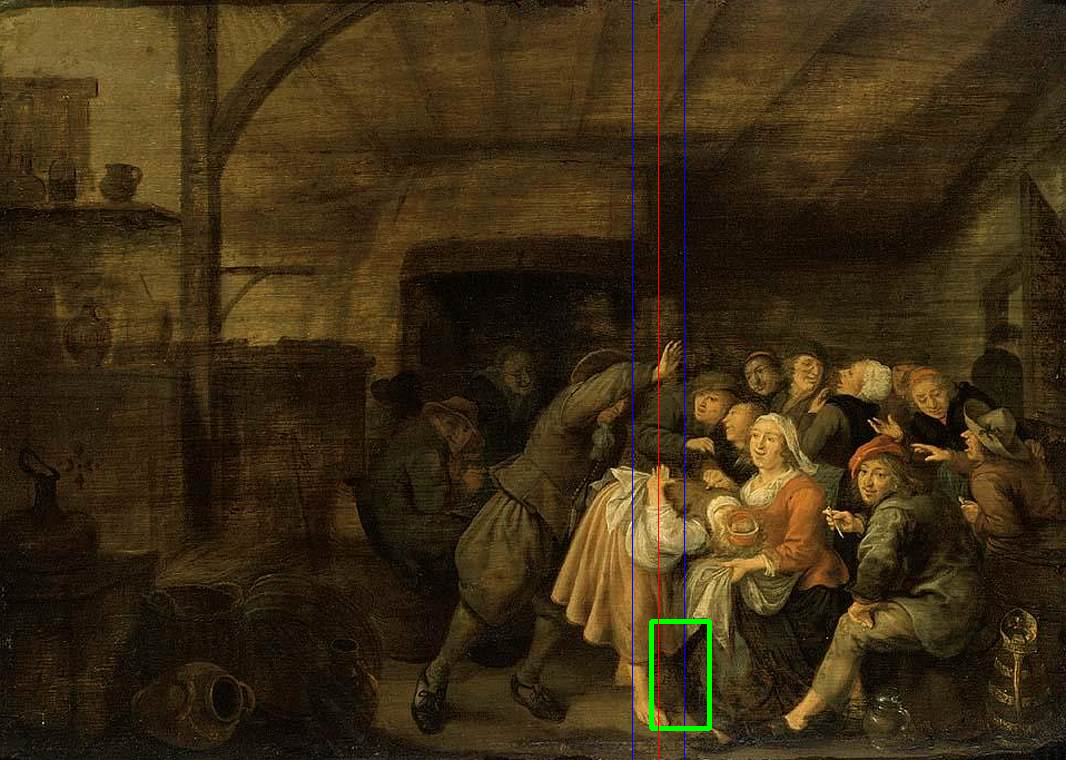
\includegraphics[scale=0.3,angle=0]{afsnit/afprovning/billeder/naive_losning/naiv_virker_ikke1.png}
	\end{center}
	\caption[]{Malerie hvor udtrækningen af regioner ikke virker, den naive
	løsning godtager en region som ligger helt forkert. Navn:
	Peasants in an Inn Playing "La Main Chaude". År: Ukendt. Af:
	Molenaer, Jan Miense.}
	\label{naiv_virker_ikke1}
\end{figure}

\begin{figure}[h!!]
	\begin{center}
		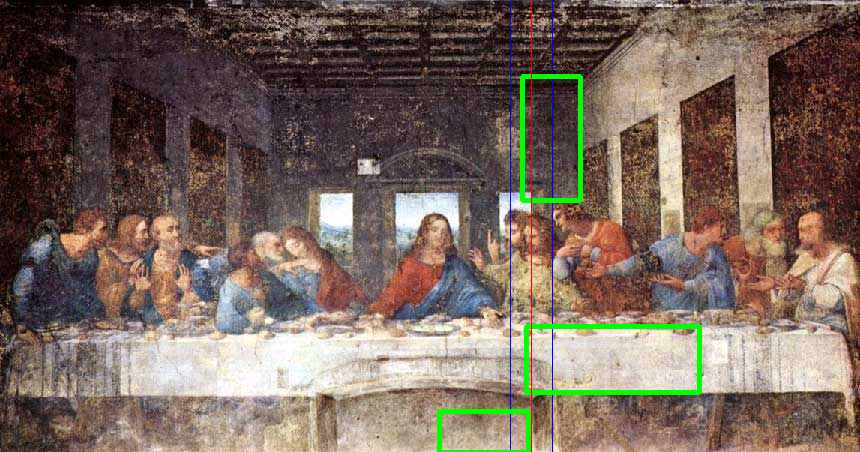
\includegraphics[scale=0.3,angle=0]{afsnit/afprovning/billeder/naive_losning/naiv_virker_ikke2.png}
	\end{center}
	\caption[]{Tre regioner bliver godtaget, selv om de ikke er særlige
	interessante.}
	\label{naiv_virker_ikke2}
\end{figure}

\begin{figure}[h!!]
	\begin{center}
		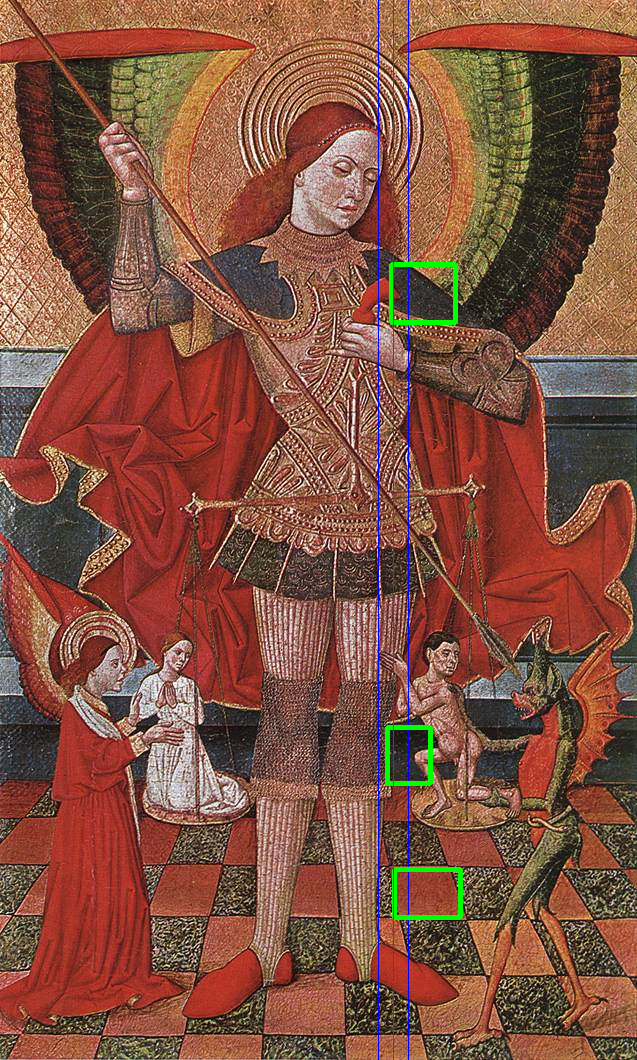
\includegraphics[scale=0.3,angle=0]{afsnit/afprovning/billeder/naive_losning/naiv_virker_ikke3.png}
	\end{center}
	\caption[]{Der bliver fundet tre regioner, hvor kun en af dem reelt passer
	på en ting i billedet.}
	\label{naiv_virker_ikke3}
\end{figure}
\clearpage

For at give et bedre overblik på hvor mange regioner vi mener er
interessante og hvor mange der er falske positive, har vi optalt dem på
de samme ni malerier som vi brugte til tærskelværdiafprøvningen. I tabel
\ref{naiv_good} kan ses antallet af interessante regioner og i tabel
\ref{naiv_bad} kan ses antallet af falske positive. Der bliver fundet 12
interessante regioner og 10 falske positive, det vil sige at der er $20
\%$ flere interessante region end falske.

\begin{table}[H]
    \centering
    \begin{tabular}{|c|l|l|l|}
			\hline
            & Kraftige farver & Medium farver & Svage farver \\\hline
		Mange detaljer	& 2 & 0 & 7 \\\hline
        Medium detaljer  & 1 & 0 & 0 \\\hline
        Få detaljer     & 1 & 0 & 1 \\\hline
    \end{tabular}
    \caption[]{Tabel over antal interessante regioner fundet i ni testmalerier i to gyldne snit.}
    \label{naiv_good}
\end{table}

\begin{table}[H]
    \centering
    \begin{tabular}{|c|l|l|l|}
			\hline
            & Kraftige farver & Medium farver & Svage farver \\\hline
		Mange detaljer	& 3 & 0 & 0 \\\hline
        Medium detaljer  & 0 & 3 & 0 \\\hline
        Få detaljer     & 1 & 3 & 0 \\\hline
    \end{tabular}
    \caption[]{Tabel over antal falske positiver i ni testmalerier i to gyldne snit.}
    \label{naiv_bad}
\end{table}

\subsection{Konklusion}
Det naive løsning virker efter intentionen på vores testbillederne, med
ensfarvet regioner, men i praksis finder den mange regioner som vi helst
ville være foruden som f.eks i maleri \ref{naiv_virker_ikke3}. På
afprøvnings malerierne findes der altså kun $20\%$ flere interessante
regioner, som vi finder korrekt detekteret end falske positiver, der er
ikke særlige godt og kommer desværre til at påvirke de resultater vi
kommer frem til.
